\chapter{Evaluation}
\label{ch:eval}

This chapter presents an empirical evaluation of the proposed architecture. The primary objective is to assess whether tracking indirect control flow through a secondary coverage map yields tangible improvements in path discovery and overall fuzzing efficacy when compared to standard techniques.

To evaluate the system, we compare the baseline AFL++ fuzzer against our modified architecture across a diverse set of real-world benchmarks, chosen for their varying levels of reliance on indirect branching. The evaluation is structured to address the core performance and coverage metrics that define a fuzzer's success.

\section{Experimental Setup}

This section outlines the hardware environment, the selected target programs, the fuzzer configurations under test, and all other parameters concerning the fuzzing campaign.

\subsection{Methodology and Environment}

All fuzzing campaigns were executed on a dedicated server running Ubuntu 24.04.4 LTS. The machine is equipped with a 64-core Intel Xeon Silver 4316 processor operating at 2.30GHz and 64GB of RAM.

To ensure the evaluation reflects real-world conditions, we selected a diverse set of targets taken from the FuzzBench repository, alongside a Ruby parser. The selected benchmarks are: 
\begin{itemize}
    \item \texttt{libxslt}
    
    \item \texttt{openssl}
    
    \item \texttt{sqlite3}
    
    \item \texttt{systemd-link-parser}
    
    \item \texttt{mruby}
\end{itemize}

These targets were deliberately chosen for their reliance on complex parsing logic and frequent use of indirect branches, which makes them ideal candidates for testing the efficacy of the proposed indirect coverage map. The inclusion of \texttt{mruby}, a lightweight Ruby implementation, further stresses the fuzzer's ability to navigate the complex indirect jumps typically found in interpreters --- e.g., in the dispatch loop.

\paragraph{Fuzzer Configurations} The analysis was conducted by comparing the standard configuration of AFL++ and our custom AFL++ architecture. The latter was tested in three different configurations: with slot sizes of 32, 64, and 128 bits.

All targets were compiled with the \texttt{afl-clang-fast} wrapper, ensuring all performance or coverage deviations can be attributed to the newly introduced mechanism.

\paragraph{Campaign Parameters} Fuzzing is inherently stochastic; therefore, single-run measurements are insufficient for drawing robust conclusions. For our campaign, each target version was fuzzed for 24 hours, restricted to a single core per run. To ensure statistical significance and account for randomness, we performed 5 independent trials per target version.

\section{Edge Coverage and Path Discovery}

This section presents the primary metrics used to evaluate the efficiency of the proposed modifications: total region coverage and queue size. We compare the standard AFL++ baseline with the modified versions across all targets.

\subsubsection{Total Edge Coverage}

The primary indicator of a fuzzer's overall success is the total number of unique code regions discovered over time. To measure this, coverage analysis was performed using \texttt{llvm-cov}. For each campaign, we gathered the inputs saved in the fuzzer's queue and replayed them against an \texttt{llvm-cov}-instrumented binary. By ordering the queue inputs by creation timestamp, we computed the cumulative region coverage over the 24-hour fuzzing campaigns.

The following plots illustrate the average region coverage growth for each benchmark over 24 hours.

% --- PAGE 1 ---
\begin{figure}[htbp]
    \centering

    \begin{subfigure}{\textwidth}
        \centering
        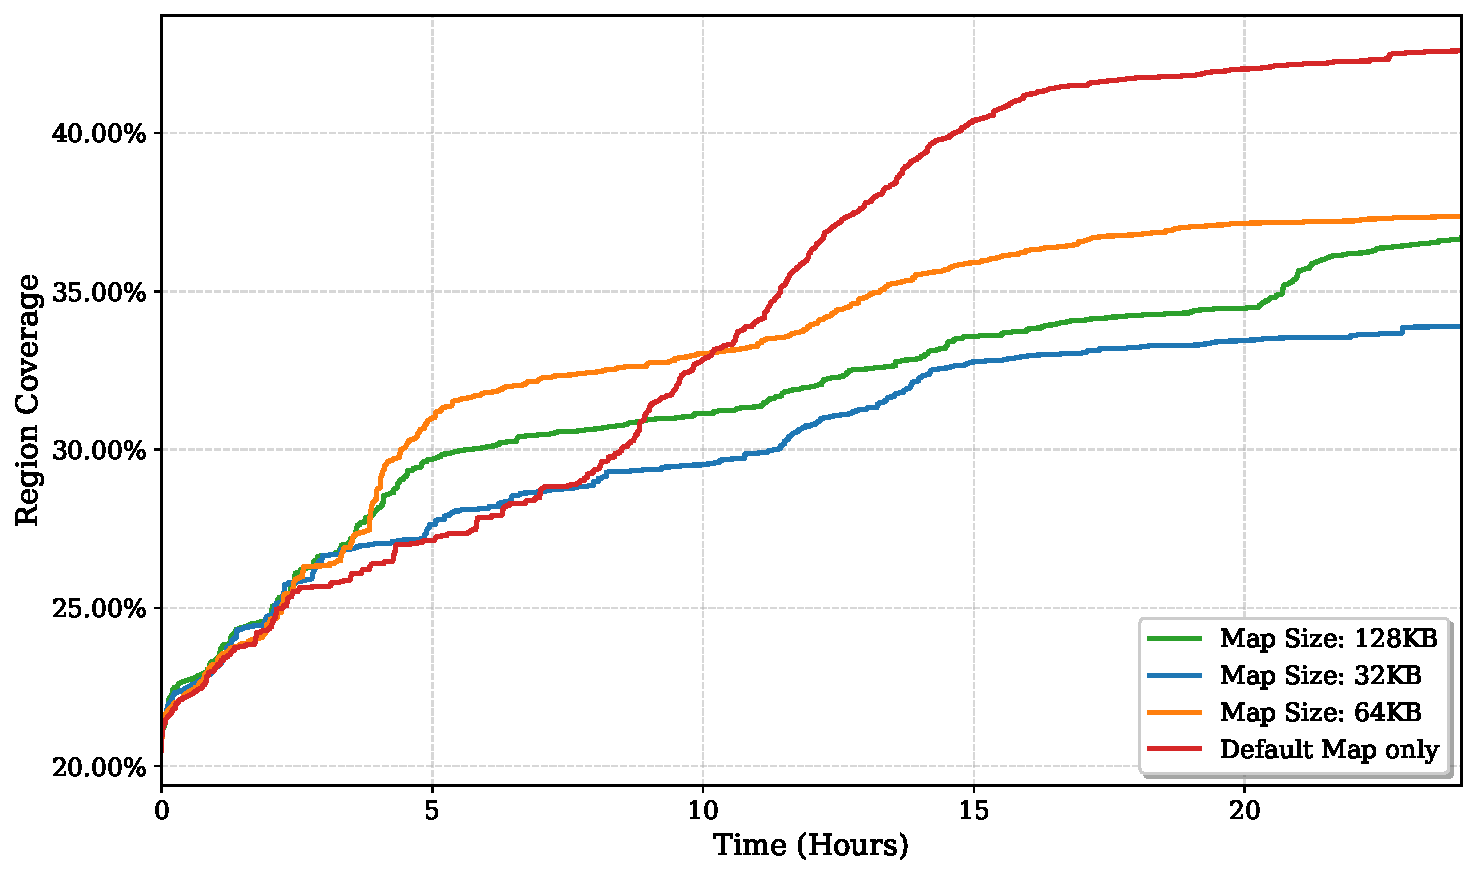
\includegraphics[width=0.85\linewidth]{imgs/eval/coverage_plot_mruby.pdf}
        \caption{mruby}
        \label{fig:plot_mruby}
    \end{subfigure}

    \vspace{2em} 

    \begin{subfigure}{\textwidth}
        \centering
        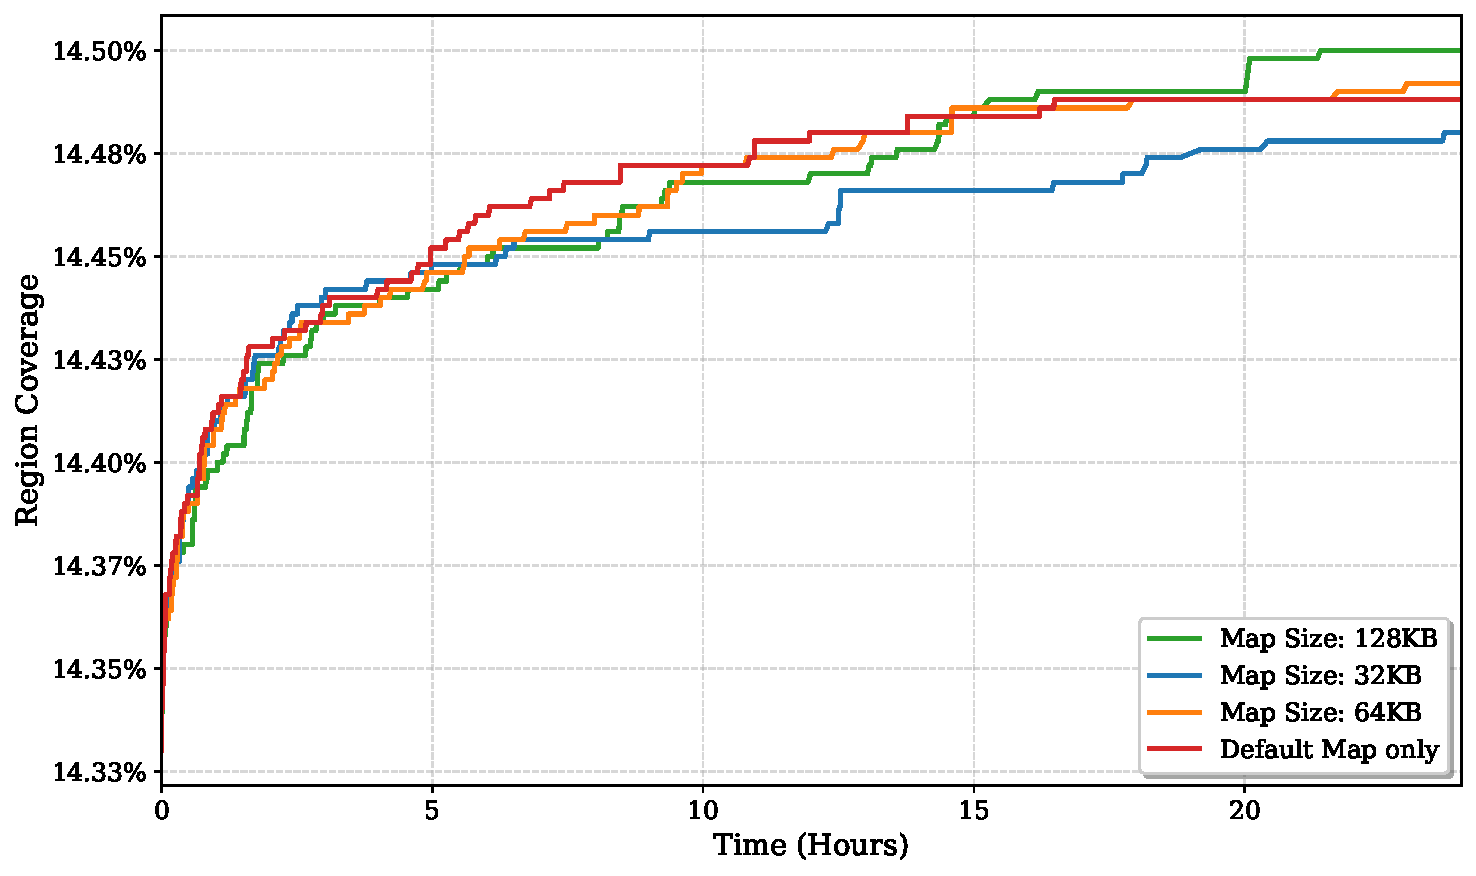
\includegraphics[width=0.85\linewidth]{imgs/eval/coverage_plot_openssl.pdf}
        \caption{OpenSSL}
        \label{fig:plot_openssl}
    \end{subfigure}

    \caption{Coverage over 24 hours for various fuzzing targets (Part 1).}
\end{figure}

% --- PAGE 2 OF THE FIGURE ---
\begin{figure}[htbp]
    \ContinuedFloat % This keeps the figure number the same
    \centering

    \begin{subfigure}{\textwidth}
        \centering
        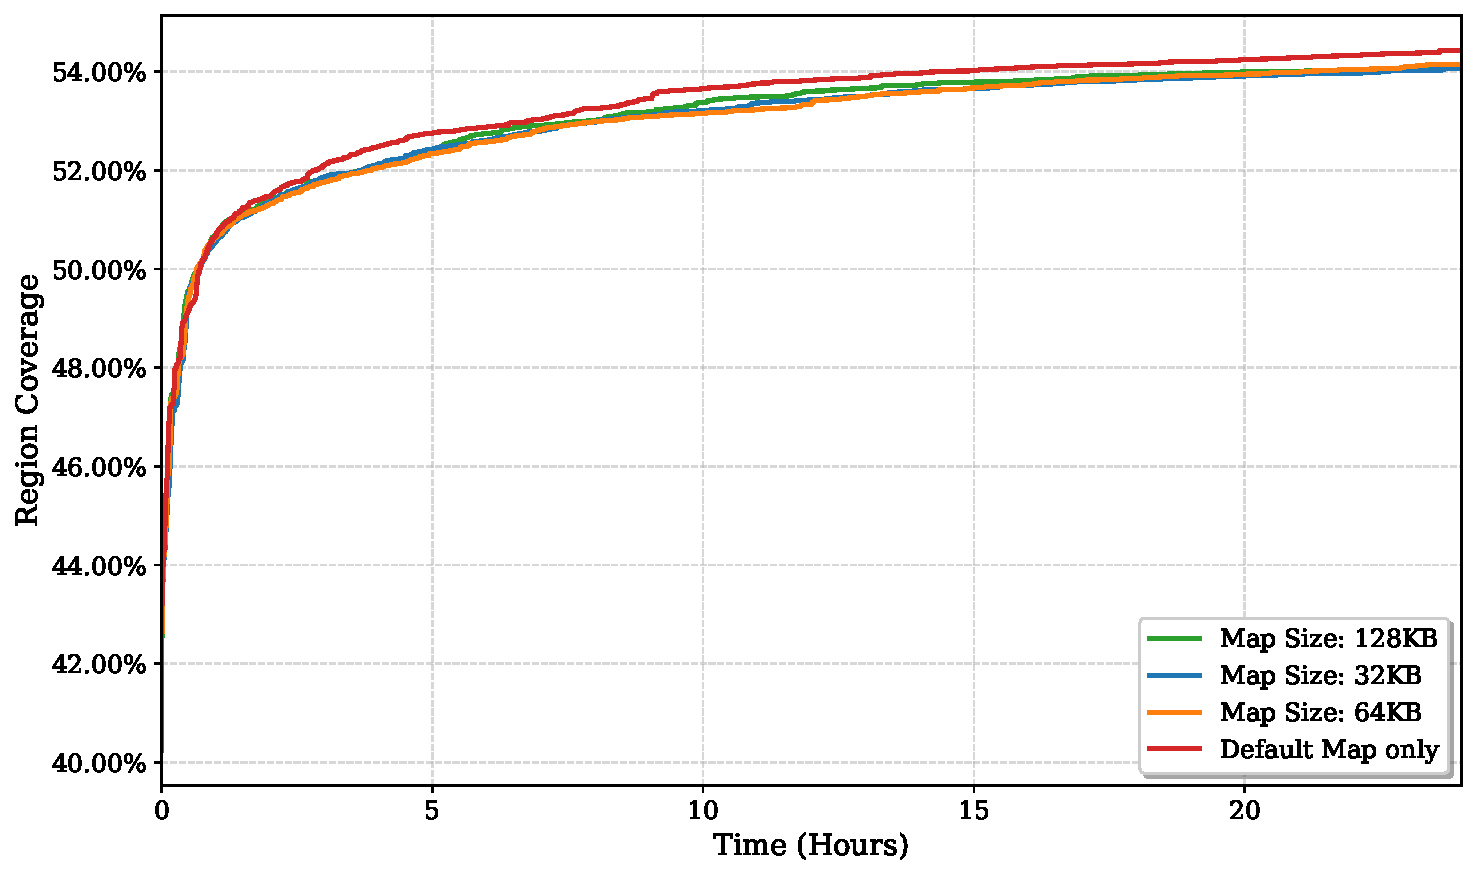
\includegraphics[width=0.85\linewidth]{imgs/eval/coverage_plot_libxslt.pdf}
        \caption{libxslt}
        \label{fig:plot_libxslt}
    \end{subfigure}
    
    \vspace{2em}

    \begin{subfigure}{\textwidth}
        \centering
        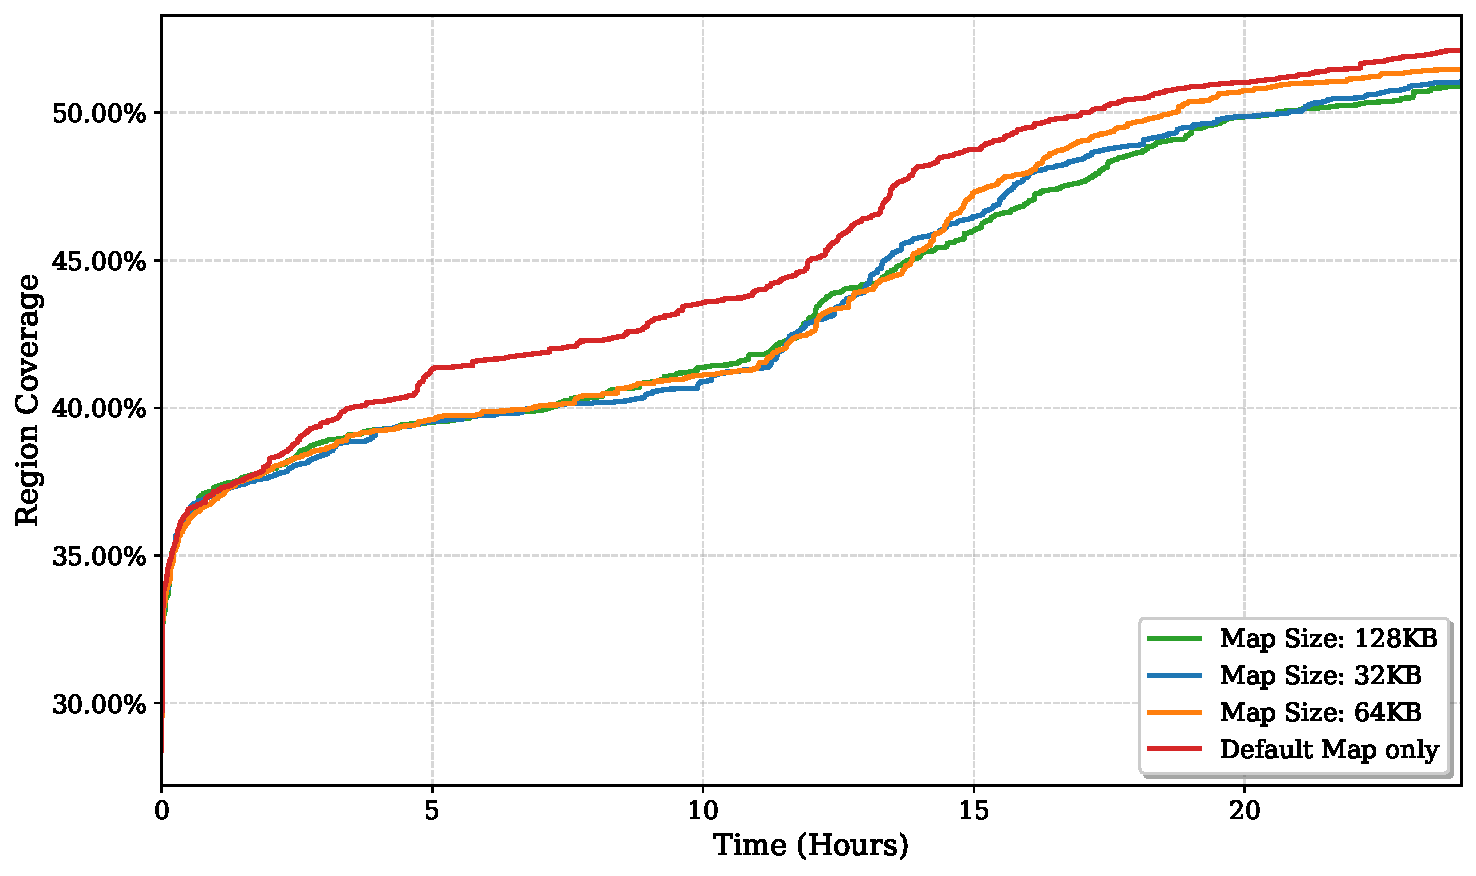
\includegraphics[width=0.85\linewidth]{imgs/eval/coverage_plot_sqlite3.pdf}
        \caption{SQLite3}
        \label{fig:plot_sqlite3}
    \end{subfigure}
    
    \caption{Coverage over 24 hours for various fuzzing targets (Part 2).}
\end{figure}


\begin{figure}[htbp]
    \ContinuedFloat % This keeps the figure number the same
    \centering

    \begin{subfigure}{\textwidth}
        \centering
        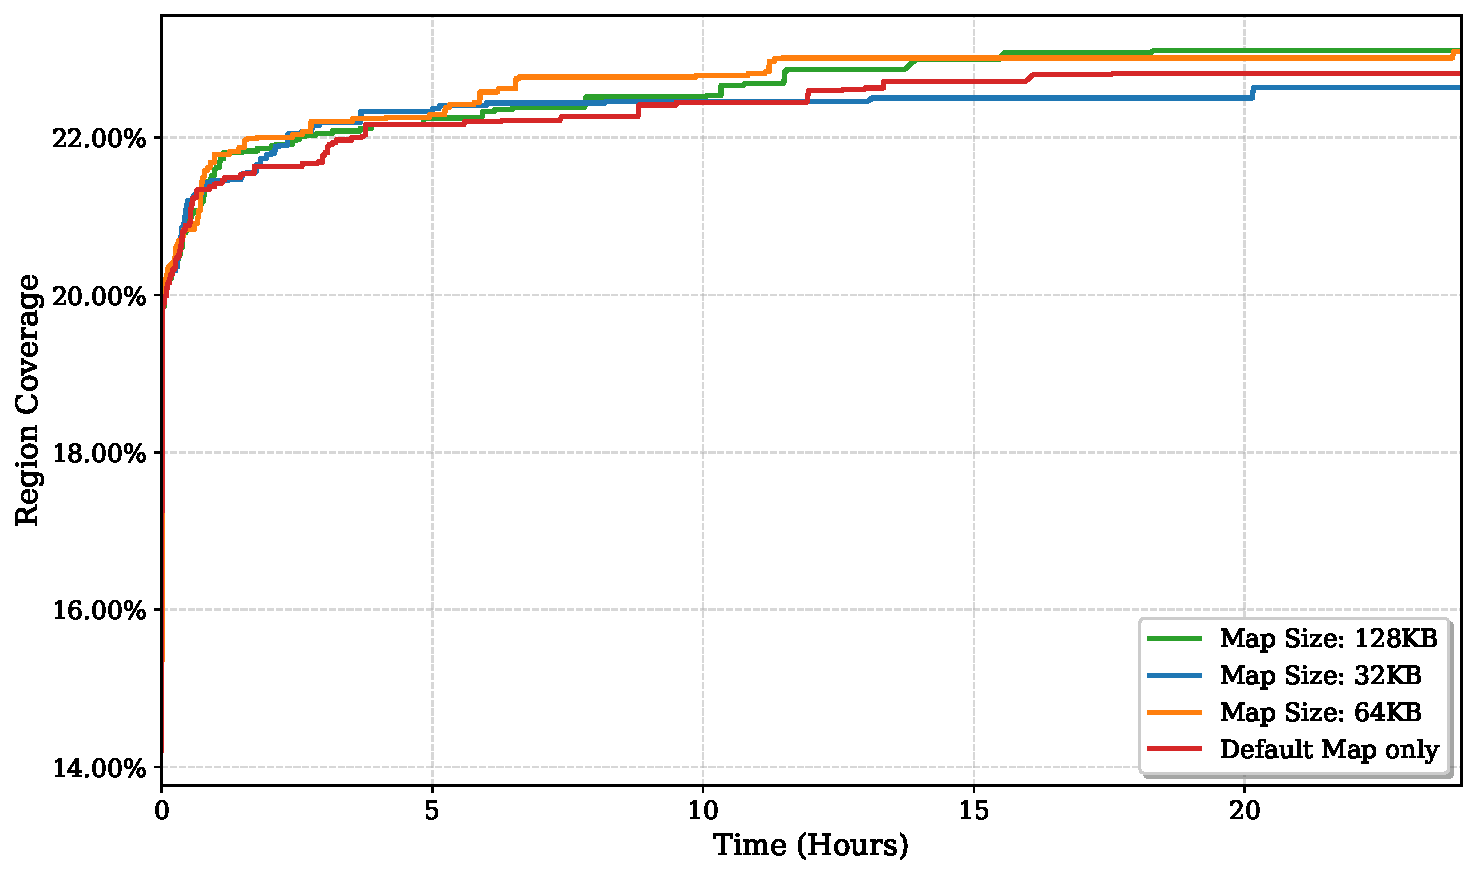
\includegraphics[width=0.85\linewidth]{imgs/eval/coverage_plot_systemd.pdf}
        \caption{systemd}
        \label{fig:plot_systemd}
    \end{subfigure}

    \caption{Coverage over 24 hours for various fuzzing targets (Part 3).}
    \label{fig:cov_plots} % The main label 
\end{figure}

\newpage

The results reveal that, across all tested benchmarks, the modified fuzzer configurations did not achieve a breakthrough in path discovery. In fact, the baseline AFL++ consistently performed either on par with or slightly better than the modified versions in terms of discovered regions within the given time frame.

Table \ref{tab:region_coverage} shows the cumulative region coverage at the end of the campaign for each target and configuration.

\begin{table}[htbp]
    \centering
    \begin{tabular}{@{}l cccc @{}}
        \toprule
        & \multicolumn{4}{c}{\textbf{Fuzzer Configuration}} \\
        \cmidrule(l){2-5}
        \textbf{Target} & \textbf{32 bit} & \textbf{64 bit} & \textbf{128 bit} & \textbf{Default} \\
        \midrule
        \textbf{libxslt} & 54.06\% & 54.14\% & 54.06\% & 54.43\% \\
        \textbf{mruby}   & 33.89\% & 37.36\% & 36.70\% & 42.61\% \\
        \textbf{openssl} & 14.48\% & 14.49\% & 14.50\% & 14.48\% \\
        \textbf{sqlite3} & 51.04\% & 51.46\% & 50.88\% & 52.11\% \\
        \textbf{systemd} & 23.10\% & 23.57\% & 23.58\% & 23.29\% \\
        \bottomrule
    \end{tabular}
    \caption{Average Region Coverage after 24 Hours}
    \label{tab:region_coverage}
\end{table}

Variations across configurations are generally minor. The 32-bit configuration more consistently results in the lowest region coverage among the modified setups. This can be attributed to a higher probability of collisions within the smaller Bloom filter, which saturates prematurely. The 64-bit and 128-bit configurations performed marginally better; however, they consistently failed to outperform the vanilla AFL++ baseline.

\subsubsection{Corpus Size}

The fuzzer's corpus (or queue) size indicates the number of unique "interesting" test cases retained during the campaign. A steadily growing queue typically indicates the continuous discovery of new paths.

The final queue sizes at the end of the campaigns are summarised in Table \ref{tab:corpus_sizes}.

\begin{table}[htbp]
\centering
\begin{tabular}{lrrrr}
\toprule
& \multicolumn{4}{c}{\textbf{Fuzzer Configuration}} \\
\cmidrule(l){2-5}
\textbf{Target} & \textbf{32 bit} & \textbf{64 bit} & \textbf{128 bit} & \textbf{Default} \\
\midrule
\textbf{libxslt} & 17,509.20 & 17,751.60 & 17,504.60 & 18,127.00 \\
\textbf{mruby}   & 5,881.40  & 8,414.80  & 7,381.00  & 11,122.80 \\
\textbf{openssl} & 2,909.20  & 2,916.40  & 2,935.80  & 2,931.00 \\
\textbf{sqlite3} & 11,054.40 & 10,761.80 & 9,875.80  & 13,026.00 \\
\textbf{systemd} & 2,173.40  & 2,125.80  & 2,171.00  & 2,261.00 \\
\bottomrule
\end{tabular}
\caption{Average Corpus Sizes after 24 Hours}
\label{tab:corpus_sizes}
\end{table}

The queue size dynamics closely mirror the region coverage data. Across all targets, the baseline AFL++ and the modified configurations maintain similar queue sizes.

This strongly implies that the indirect map rarely triggered additional seed saves. When an indirect branch was resolved dynamically, the input was almost always already flagged as "interesting" by the primary coverage map.

\section{Performance Overhead}

While the primary goal of the additional coverage map is to increase path discovery, any added instrumentation inherently risks reducing the execution throughput. A significant drop in executions per second (exec/s) can offset the benefits of better feedback. This section evaluates the computational penalty introduced by our architecture.

\subsubsection{Execution Throughput}

To assess the impact, we compared the average executions per second across all campaigns for all tested configurations.

\begin{table}[htbp]
\centering
\begin{tabular}{lrrrrr}
\toprule
& \multicolumn{4}{c}{\textbf{Fuzzer Configuration}} \\
\cmidrule(l){2-5}
\textbf{Target} & \textbf{32 bit} & \textbf{64 bit} & \textbf{128 bit} & \textbf{Default} & \textbf{Overhead} \\
\midrule
\textbf{libxslt} & 586.28 & 644.88 & 587.78 & 698.71 & +13.22\% \\ 
\textbf{mruby} & 70.10 & 75.42 & 74.82 & 79.10 & +7.15\% \\ 
\textbf{openssl} & 2732.29 & 2610.04 & 2836.24 & 3644.51 & +25.2\% \\ 
\textbf{sqlite3} & 407.75 & 424.23 & 381.44 & 452.38 & +10.59\% \\ 
\textbf{systemd} & 115.13 & 110.06 & 111.76 & 110.53 & -1.62\% \\ 
\bottomrule
\end{tabular}
\caption{Average Execs Per Second and Resulting Overhead}
\label{tab:exec_overhead}
\end{table}

Table \ref{tab:exec_overhead} shows the average execution speeds and average overhead across all configurations. 

The data indicates that the secondary map, along with all the necessary mechanisms, introduces a measurable execution penalty that varies heavily by target. Across the benchmarks, the modified fuzzer experienced overhead ranging from $7\%$ to over $25\%$ --- with the anomaly of \texttt{systemd}, which can be attributed to environmental noise and statistical margin of error. 

Targets with particularly high densities of indirect branches exhibited the worst degradation. Furthermore, a significant proportion of the overhead resides in the post-execution phase, meaning that targets with higher absolute numbers of executions per second seem to suffer greater proportional degradation.

Some of the overhead is attributable to the injection of a callback, as the routine to call a function is computationally expensive. This could be mitigated in the future by injecting LLVM IR directly instead of relying on a function call.

\section{Analysis of Results}

As established in the previous sections, the failure of the modified fuzzer to outperform the baseline cannot be solely attributed to performance overhead. The lack of improvement, despite the functional mechanism, points to structural and theoretical limitations in how fuzzers interact with indirect control flow. This section details potential reasons why the indirect coverage map did not yield the expected improvements.

\subsection{Redundancy with the Primary Edge Map}

The primary reason why the modified architecture behaves similarly to standard AFL++ is that the new map provides almost entirely redundant feedback for fully instrumented targets. 

When an indirect jump dynamically resolves to a new target block, there will almost certainly be some new direct edges to be tracked by the standard coverage map. The injected callback is invoked immediately before the indirect jump, logging the target address to the secondary map. However, immediately after the jump, the primary map still logs the new edges encountered.

Consequently, every time the secondary map reports a new target, the primary map simultaneously reports a new edge. Because the fuzzer requires only one of the maps to signal novelty to preserve the seed, the indirect map does not force the fuzzer to save any seed it would not have already discovered through standard mechanisms.

\subsection{Other Limiting Factors}

Beyond the fundamental redundancy issue, several other structural limitations prevent the secondary coverage map from driving deeper program exploration.

\subsubsection{Mutation Engine Limitations}

Discovering new indirect targets often requires the fuzzer to create specific data structures, such as memory pointers or function pointer tables. Standard mutators are effective at breaking simple conditional comparisons but are inadequate for guessing valid pointers \cite{aschermann2019redqueen, rawat2017vuzzer, wang2010taintscope}. 

Even if the secondary map is fully capable of tracking new indirect targets, the standard mutation engine might not be capable of generating the inputs required to satisfy the constraints needed to reach them without further assistance.

\subsubsection{Target Sparsity}

In many standard C/C++ benchmarks, the actual state space of possible indirect jump targets is relatively small. Once the few possible novelties for each source have been exhausted, the secondary map will never produce another "new bit" for the call site.

We observed that most sources have only one or two possible targets, with the exception of a few with significantly more --- e.g., interpreter dispatch blocks. These can be exhausted very quickly and provide minimal feedback.
